% !TeX program = pdflatex
% Plantilla institucional editable — UTEQ 
% Compatible con Overleaf usando pdfLaTeX (compilador predeterminado).
\documentclass[12pt,a4paper,oneside]{article}
\usepackage[T1]{fontenc}
\usepackage[utf8]{inputenc}
\usepackage{newtxtext,newtxmath}
% NewTX es una fuente tipo Times compatible con pdfLaTeX y Overleaf.
% Para la fuente exacta Times New Roman sería necesario usar XeLaTeX.
\usepackage[spanish,es-nodecimaldot]{babel}
\usepackage[a4paper,top=2.25cm,bottom=2.2cm,left=2.4cm,right=2.2cm,headheight=28pt]{geometry}
\usepackage{microtype}
\usepackage{graphicx}
\usepackage{float}
\usepackage{booktabs,tabularx,array,longtable}
\usepackage{enumitem}
\usepackage{xcolor}
\usepackage{tikz}
\usetikzlibrary{calc,positioning}
\usepackage[most]{tcolorbox}
\usepackage{listings}
\usepackage{fancyhdr}
\usepackage{titlesec}
\usepackage{titletoc}
\usepackage{caption}
\usepackage{subcaption}
\usepackage{hyperref}
\usepackage{setspace}
\setstretch{1.12}
\setlength{\parindent}{0pt}
\setlength{\parskip}{7pt}
\newcolumntype{Y}{>{\raggedright\arraybackslash}X}
\definecolor{azul}{HTML}{122A46}
\definecolor{azulmedio}{HTML}{254B71}
\definecolor{turquesa}{HTML}{008D95}
\definecolor{dorado}{HTML}{E2B45E}
\definecolor{tint}{HTML}{F3F7FA}
\definecolor{gris}{HTML}{566579}
\definecolor{borde}{HTML}{D8E2EB}
\definecolor{codigo}{HTML}{F7F9FC}
\definecolor{verdeorcid}{HTML}{A6CE39}
% =================== DATOS EDITABLES ===================
\newcommand{\universidad}{UNIVERSIDAD TÉCNICA ESTATAL DE QUEVEDO}
\newcommand{\facultad}{FACULTAD DE CIENCIAS DE LA COMPUTACIÓN}
\newcommand{\carrera}{CARRERA DE INGENIERÍA DE SOFTWARE}
\newcommand{\materia}{Administración de Base de Datos}
\newcommand{\tema}{Barbershop: primera versión funcional y consolidación de la documentación del proyecto integrador}
\newcommand{\orcidlink}[1]{\href{https://orcid.org/#1}{\tikz[baseline=-0.15em]{\node[circle,fill=verdeorcid,inner sep=1.5pt,text=white,font=\sffamily\bfseries\tiny]{iD};}\enspace\textcolor{black}{\small #1}}}
\newcommand{\estudiante}{{\renewcommand{\arraystretch}{1.15}\begin{tabular}[t]{@{}l@{\hspace{0.8em}}l@{}}
Amagua Sacón Robyn Willian & \orcidlink{0009-0006-7363-4276}\\
Barrionuevo Fuentes Carlos Daniel & \orcidlink{0009-0003-3415-3208}\\
Marcillo Ponce Alberto Jeanpool & \orcidlink{0009-0003-7886-3957}\\
Mesías Quijije Jhon Alexander & \orcidlink{0009-0001-6929-7514}\\
Vera Gómez Anthony Alfredo & \orcidlink{0009-0007-8198-6199}
\end{tabular}}}
\newcommand{\docente}{Ing. Cordero Bazurto José Steven}
\newcommand{\orcidestudiante}{0000-0000-0000-0000} % Reemplace con su ORCID real
\newcommand{\curso}{Quinto nivel --- Paralelo A}
\newcommand{\fechaentrega}{21 de noviembre de 2026}
\newcommand{\lugar}{Quevedo -- Ecuador}
\newcommand{\anio}{2026}
% Colocar el escudo en logos/logo-uteq.png (carpeta logos junto al .tex).
% Si no existe, se muestra un monograma decorativo.
\newcommand{\logoinstitucional}{%
  \IfFileExists{logos/logo-uteq.png}{
\includegraphics[height=3.1cm,keepaspectratio]{logos/logo-uteq.png}}{%
    \begin{tikzpicture}\draw[turquesa,line width=1.5pt] (0,0) circle (1.12);
    \node[font=\bfseries\Large,text=azul] at (0,0) {UTEQ};\end{tikzpicture}}}
\newcommand{\orcidperfil}{\href{https://orcid.org/\orcidestudiante}{\tikz[baseline=-0.15em]{\node[circle,fill=verdeorcid,inner sep=1.8pt,text=white,font=\sffamily\bfseries\scriptsize]{iD};}\enspace\textcolor{black}{\orcidestudiante}}}
% Numeraciones con punto final: 1. Introducción / 2.1. Objetivo general
\renewcommand{\thesection}{\arabic{section}.}
\renewcommand{\thesubsection}{\arabic{section}.\arabic{subsection}.}
\renewcommand{\thesubsubsection}{\arabic{section}.\arabic{subsection}.\arabic{subsubsection}.}
\hypersetup{unicode=true,colorlinks=true,linkcolor=black,urlcolor=black,citecolor=black,pdftitle={\tema},pdfauthor={Amagua Robyn; Barrionuevo Carlos; Marcillo Alberto; Mes\'ias Jhon; Vera Anthony}}
\addto\captionsspanish{\renewcommand{\contentsname}{Contenido}\renewcommand{\listfigurename}{Índice de figuras}\renewcommand{\listtablename}{Índice de tablas}}
\titleformat{\section}{\Large\bfseries\color{black}}{\thesection}{0.8em}{}
\titleformat{\subsection}{\large\bfseries\color{black}}{\thesubsection}{0.75em}{}
\titleformat{\subsubsection}{\normalsize\bfseries\color{black}}{\thesubsubsection}{0.7em}{}
\titlespacing*{\section}{0pt}{19pt}{10pt}
\titlespacing*{\subsection}{0pt}{13pt}{5pt}
\titlecontents{section}[0em]{\vspace{4pt}\bfseries\color{black}}{\contentslabel{2.2em}}{}{\titlerule*[0.6pc]{.}\contentspage}
\captionsetup{font=small,labelfont={bf,color=black},labelsep=period}
\pagestyle{fancy}\fancyhf{}
\fancyhead[L]{\small\textbf{UTEQ}\enspace|\enspace Ingeniería de Software}
\fancyhead[R]{\small Informe técnico --- Barbershop V1.1}
\renewcommand{\headrulewidth}{0.6pt}
\renewcommand{\headrule}{\hbox to\headwidth{\color{borde}\leaders\hrule height \headrulewidth\hfill}}
\fancyfoot[C]{\small\thepage}
\renewcommand{\footrulewidth}{0pt}
\newtcolorbox{destacado}[1][]{enhanced,breakable,colback=tint,colframe=borde,boxrule=.6pt,arc=2mm,
  borderline west={3pt}{0pt}{turquesa},left=13pt,right=11pt,top=9pt,bottom=9pt,#1}
\newtcolorbox{resultado}[1][]{enhanced,breakable,colback=white,colframe=turquesa!55,boxrule=.75pt,arc=2mm,
 title={\bfseries Resultado o hallazgo},coltitle=black,colbacktitle=tint,#1}
\lstdefinestyle{estiloUTEQ}{backgroundcolor=\color{codigo},basicstyle=\ttfamily\footnotesize,
  keywordstyle=\color{black}\bfseries,commentstyle=\color{black}\itshape,
  stringstyle=\color{black},numbers=left,numberstyle=\tiny\color{black},
  numbersep=10pt,stepnumber=1,frame=single,rulecolor=\color{borde},framesep=8pt,
  breaklines=true,breakatwhitespace=false,showstringspaces=false,tabsize=2,
  keepspaces=true,columns=fullflexible,captionpos=b,xleftmargin=7pt,xrightmargin=3pt}
\lstset{style=estiloUTEQ}
\renewcommand{\lstlistingname}{Código}
\renewcommand{\lstlistlistingname}{Índice de códigos}
% Recuadro para una fotografía aún no disponible. Sustituir por \includegraphics.
\newcommand{\imagenplaceholder}[1]{\begin{tikzpicture}
 \node[draw=borde,fill=tint,rounded corners=3pt,minimum width=.89\linewidth,
 minimum height=5.4cm,align=center,text=black,font=] {\Large\bfseries Evidencia fotográfica\\[6pt]\normalsize #1\\[7pt]\small Reemplazar con \texttt{\textbackslash includegraphics}};
 \end{tikzpicture}}
\begin{document}
% ========================= PORTADA =========================
\begin{titlepage}
\begin{tikzpicture}[remember picture,overlay]
  \fill[azul] (current page.north west) rectangle ([yshift=-1.05cm]current page.north east);
  \fill[turquesa] ([yshift=-1.05cm]current page.north west) rectangle ([yshift=-1.12cm]current page.north east);
  \fill[azul] ([yshift=1.05cm]current page.south west) rectangle (current page.south east);
  \fill[dorado] ([xshift=1.8cm,yshift=1.05cm]current page.south west) rectangle
  ([xshift=5.7cm,yshift=1.12cm]current page.south west);
\end{tikzpicture}
\vspace*{0.35cm}
\begin{center}
\logoinstitucional\\[0.55cm]
{\normalsize\bfseries\color{black}\universidad}\\[0.16cm]
{\small\color{black}\facultad}\\[0.12cm]
{\small\bfseries\color{black}\carrera}
\end{center}
\vspace{1.25cm}
\begin{center}
{\small\bfseries\color{black}\MakeUppercase{INFORME TÉCNICO}}\\[0.48cm]
{\fontsize{19}{23}\selectfont\bfseries\color{black}\tema}\\[0.65cm]
{\color{dorado}\rule{3.7cm}{2pt}}\\[0.35cm]
{\large\color{black}\materia}
\end{center}
\vfill
\begin{tcolorbox}[colback=tint,colframe=borde,arc=2mm,boxrule=.7pt,left=15pt,right=15pt,top=12pt,bottom=12pt]
% Ambas columnas centradas verticalmente para alinear etiqueta y valor.
\renewcommand{\arraystretch}{1.75}
\begin{tabular}{@{}>{\bfseries\raggedright\arraybackslash}m{3.1cm}>{\raggedright\arraybackslash}m{10.7cm}@{}}
Equipo: & \estudiante\\
Docente: & \docente\\
Curso: & \curso\\
Entrega: & \fechaentrega\\
Repositorio: & \href{https://github.com/ramaguas-ship-it/Barbershop}{\textcolor{azul}{\small github.com/ramaguas-ship-it/Barbershop}}
\end{tabular}
\end{tcolorbox}
\vspace{0.65cm}
\begin{center}{\bfseries\color{black}\lugar\quad |\quad\anio}\end{center}
\vspace{0.35cm}
\end{titlepage}
% ========================= PRELIMINARES =========================
\pagenumbering{roman}
\setcounter{page}{1}
\tableofcontents
\clearpage
% Activar estos índices si el documento contiene varias figuras o tablas:
% \listoffigures\clearpage
% \listoftables\clearpage
% \lstlistoflistings\clearpage
\pagenumbering{arabic}
% ===== CUERPO =====
\section{Documentaci\'on general del proyecto}
\subsection{Misi\'on}
Reemplazar el cuaderno y los mensajes con los que una barber\'ia de una sola sucursal lleva su agenda por una aplicaci\'on web con PostgreSQL, de modo que cada barbero tenga un horario sin cruces, el negocio conozca qu\'e citas, cobros, cajas y existencias tiene, y el cliente reserve sin repetir sus datos.

\subsection{Stakeholders}
\begin{table}[H]\centering\small
\begin{tabularx}{\textwidth}{>{\raggedright\arraybackslash}p{3.2cm}YY}\toprule
\textbf{Stakeholder} & \textbf{Inter\'es en el proyecto} & \textbf{Relaci\'on con el sistema}\\\midrule
Propietario / administrador & Controlar servicios, precios, barberos, caja e inventario; reducir p\'erdidas por faltantes sin responsable. & Usuario con rol \emph{administrador}; aprueba devoluciones y revisa diferencias de caja (V1.2).\\
Barberos & Conocer su agenda y registrar su trabajo sin cruces ni disputas por horarios. & Usuarios con rol \emph{barbero}; consultan su agenda y cambian el estado de sus citas.\\
Clientes & Reservar, reprogramar o cancelar sin llamadas ni repetir datos; pagar en l\'inea (V1.1 posterior). & Usuarios con rol \emph{cliente}; se registran una sola vez.\\
Pasarela de pago (externa) & Procesar los pagos en l\'inea. & Sistema externo; su integraci\'on (RF-08) a\'un no est\'a implementada.\\
Servicio de correo (externo) & Entregar confirmaciones y avisos. & Sistema externo; previsto en V1.2 (RF-21).\\
Docente evaluador & Verificar integraci\'on con PostgreSQL, pruebas y trazabilidad. & Revisa el informe, el c\'odigo y los scripts entregados.\\
Equipo de desarrollo (5 integrantes) & Entregar una V1 funcional dentro del semestre. & Dise\~na, implementa, prueba y documenta.\\\bottomrule
\end{tabularx}
\caption{Stakeholders de Barbershop}\end{table}

\subsection{Objetivos}
\textbf{Objetivo general.} Desarrollar la versi\'on 1 de una aplicaci\'on web que gestione citas (con y sin reserva previa), cobros (incluido el pago en l\'inea), la caja de cada barbero y el inventario de una barber\'ia, usando PostgreSQL como gestor de base de datos.

\textbf{Objetivos espec\'ificos} (mantenidos de la especificaci\'on de la semana 2; entre par\'entesis, su situaci\'on actual):
\begin{itemize}[nosep]
\item Permitir que los clientes se registren una sola vez y reserven, reprogramen o cancelen citas sin cruces de horario (\textbf{alcanzado en V1.1}: RF-01 a RF-06).
\item Atender a los clientes sin cita mediante una cola de turnos y liberar los horarios de los ausentes (pendiente: RF-14 a RF-17).
\item Ofrecer el pago en l\'inea con devoluci\'on aprobada por el administrador (pendiente: RF-08, RF-68).
\item Registrar servicios cobrados y productos vendidos (pendiente: RF-09).
\item Controlar la caja individual de cada barbero con arqueo y faltantes (pendiente: RF-41, RF-25, RF-26).
\item Controlar el inventario con descuento autom\'atico y alertas (pendiente: RF-10, RF-11).
\item Preparar la atenci\'on de fechas de alta demanda (pendiente: RF-28, RF-29).
\end{itemize}
No se modificaron objetivos ni alcance en esta etapa; solo se prioriz\'o el orden de implementaci\'on.

\subsection{Alcance}
\textbf{Incluido en el semestre (V1):} una sola sucursal; clientes registrados y clientes sin cita; citas con reprogramaci\'on, cancelaci\'on y tiempo de gracia; servicios, barberos y horarios; cobros (efectivo, transferencia, tarjeta en local y pago en l\'inea); caja individual con arqueo; inventario; fechas de alta demanda; correos de confirmaci\'on.

\textbf{Implementado en esta entrega (V1.1 parcial):} autenticaci\'on por roles, registro y perfil del cliente, CRUD de servicios y barberos, reserva con validaci\'on de disponibilidad, reprogramaci\'on y cancelaci\'on, y agenda del barbero con cambio de estado.

\textbf{Excluido de forma definitiva:} facturaci\'on electr\'onica del SRI, comisiones, multisucursal, aplicaci\'on m\'ovil nativa, fidelizaci\'on, precios din\'amicos y chatbot.

\subsection{Limitaciones}
\begin{itemize}[nosep]
\item \textbf{T\'ecnicas:} horario de atenci\'on global (08:00--18:00, configurable por variable de entorno) y no por barbero (RF-19 pendiente); sin pasarela de pago, correo ni cola de turnos; sin recuperaci\'on de contrase\~na (parte de RNF-20); HTTPS no configurado en desarrollo; una cita pagada no puede modificarse hasta contar con devoluciones (RF-68).
\item \textbf{Temporales:} el semestre acota la V1; por eso se divide en V1.1 (n\'ucleo) y V1.2 (caja, alta demanda, correo).
\item \textbf{Econ\'omicas:} la pasarela de pago y el despliegue deben usar entornos de prueba o servicios gratuitos.
\item \textbf{De recursos:} cinco integrantes con distinto dominio de Node.js y SQL; un solo servidor PostgreSQL local en Docker; las pruebas de esta entrega se ejecutaron sobre PostgreSQL 16.15, mientras que el contenedor del equipo usa PostgreSQL 18 (ver secci\'on de dificultades).
\end{itemize}

\subsection{Riesgos potenciales}
\begin{table}[H]\centering\small
\begin{tabularx}{\textwidth}{>{\raggedright\arraybackslash}p{0.5cm}>{\raggedright\arraybackslash}p{3.2cm}YY}\toprule
\textbf{N.\textdegree} & \textbf{Riesgo} & \textbf{Posible consecuencia} & \textbf{Medida de prevenci\'on o mitigaci\'on}\\\midrule
1 & Reservas simult\'aneas del mismo horario para un barbero & Dos clientes con la misma cita; conflictos en el local & Restricci\'on \texttt{EXCLUDE} en PostgreSQL (RN-01, RNF-13); comprobada con 20 solicitudes simult\'aneas (PF-22)\\
2 & P\'erdida de datos al eliminar o recrear el contenedor Docker & P\'erdida de citas, clientes y precios & Volumen nombrado \texttt{pgdata\_abd}; respaldo diario con \texttt{pg\_dump} y prueba de restauraci\'on (RNF-06)\\
3 & Dependencia de una pasarela de pago externa (RF-08) & Estados de pago inconsistentes o integraci\'on bloqueada & Dejarla para el final de V1.1; usar entorno de pruebas; guardar solo referencia, monto y estado (RNF-09, RNF-10)\\
4 & Faltantes de caja sin responsable por implementar tarde el control de caja & P\'erdidas econ\'omicas sin trazabilidad & Priorizar RF-41 al inicio de la siguiente etapa; reglas RN-03 a RN-07 como restricciones de BD\\
5 & Exposici\'on de datos personales de clientes (LOPDP) & Sanciones y p\'erdida de confianza & Consentimiento obligatorio en el registro, contrase\~nas con bcrypt, token CSRF, sesi\'on de 30 minutos, HTTPS en producci\'on y ning\'un dato de tarjeta almacenado\\
6 & Desfase entre integrantes (ramas, scripts SQL o versiones distintas de PostgreSQL) & Errores que solo aparecen en un equipo; esquema inconsistente & Scripts idempotentes versionados en Git, \texttt{README} con pasos reproducibles, misma imagen \texttt{postgres:18} y pruebas automatizadas con \texttt{npm test}\\
7 & Clientes que no asisten & Horarios perdidos y menor ingreso & Tiempo de gracia y estado \emph{ausente} que libera el horario (RF-17, pendiente); la restricci\'on ya excluye las citas ausentes\\\bottomrule
\end{tabularx}
\caption{Riesgos del proyecto}\end{table}

\subsection{Roles de usuarios}
\begin{table}[H]\centering\small
\begin{tabularx}{\textwidth}{>{\raggedright\arraybackslash}p{2.6cm}Y}\toprule
\textbf{Rol} & \textbf{Actividades dentro del sistema (estado actual)}\\\midrule
Administrador & Registrar, editar, desactivar y eliminar servicios (nombre, duraci\'on, precio) y barberos; consultar todas las citas y cancelarlas a solicitud del cliente. \emph{Pendiente:} horarios y feriados, inventario, aprobaci\'on de devoluciones, supervisi\'on de cajas, fechas de alta demanda.\\
Barbero & Consultar su agenda por fecha y cambiar el estado de sus citas (confirmada, en espera, en atenci\'on, atendida, ausente, cancelada) seg\'un transiciones v\'alidas; ver solo sus citas. \emph{Pendiente:} cobros, caja, cola de turnos, registro r\'apido de clientes sin cita.\\
Cliente & Registrarse una sola vez, consultar y editar su perfil, reservar citas eligiendo barbero, servicio, fecha y horario libre, y reprogramar o cancelar sus citas pendientes con un plazo m\'inimo de 2 horas. \emph{Pendiente:} pago en l\'inea y notificaciones por correo.\\\bottomrule
\end{tabularx}
\caption{Roles de usuario}\end{table}

\section{Entorno y conexi\'on con PostgreSQL}
La aplicaci\'on usa Node.js, Express 5 y la biblioteca \texttt{pg}. La conexi\'on se define con \texttt{DATABASE\_URL} y se apunta al contenedor \texttt{postgres\_abd} (imagen \texttt{postgres:18}, puerto 5432, volumen \texttt{pgdata\_abd}) administrado con DBeaver, seg\'un el manual t\'ecnico del equipo. Se cre\'o una base propia, \texttt{barbershop}, distinta de \texttt{laboratorio\_abd}. Los scripts \texttt{db/01\_schema.sql} y \texttt{db/02\_seed.sql} son repetibles y se aplican con \texttt{npm run db:init}. Todas las consultas son parametrizadas (\texttt{\$1}, \texttt{\$2}\ldots); ninguna sentencia SQL concatena datos del usuario. Las operaciones que modifican varias tablas se ejecutan en transacci\'on y registran el usuario actuante para la auditor\'ia.

\subsection{Modelo de datos}
\begin{table}[H]\centering\small
\begin{tabularx}{\textwidth}{>{\ttfamily}p{2.6cm}Y}\toprule
\textbf{Tabla} & \textbf{Contenido y restricciones principales}\\\midrule
usuarios & Cliente, barbero o administrador; correo \'unico sin distinguir may\'usculas; hash bcrypt; \texttt{CHECK} de rol y tel\'efono; intentos fallidos y bloqueo.\\
barberos & Perfil operativo 1:1 con un usuario de rol barbero; \texttt{ON DELETE RESTRICT}.\\
servicios & Nombre \'unico, duraci\'on entre 5 y 480 minutos, precio $\geq 0$.\\
citas & Cliente, barbero, servicio, \texttt{inicio}/\texttt{fin} (\texttt{timestamptz}), estado y estado de pago; \texttt{EXCLUDE} que impide solapes de citas activas del mismo barbero.\\
auditoria & Usuario, acci\'on, tabla, registro y valor anterior (JSONB) de cambios de precio y cancelaciones, mediante triggers.\\
sesiones & Almac\'en de sesiones (expiraci\'on a 30 minutos de inactividad).\\\bottomrule
\end{tabularx}
\caption{Estructura de la base de datos \texttt{barbershop}}\end{table}

\begin{lstlisting}[language=SQL,caption={Restricci\'on que aplica RN-01, RN-13 y RNF-13 en la base de datos}]
CONSTRAINT ex_citas_sin_cruce EXCLUDE USING gist (
    barbero_id WITH =,
    tstzrange(inicio, fin, '[)') WITH &&
) WHERE (estado NOT IN ('cancelada', 'ausente'))
\end{lstlisting}

\section{Funcionalidades implementadas}
\begin{table}[H]\centering\small
\begin{tabularx}{\textwidth}{>{\raggedright\arraybackslash}p{1.6cm}>{\raggedright\arraybackslash}p{3.3cm}Y}\toprule
\textbf{Requisito} & \textbf{Operaci\'on CRUD} & \textbf{Funcionalidad y validaciones}\\\midrule
RF-01 & Crear, leer, actualizar & Registro con nombre, tel\'efono, correo, contrase\~na y consentimiento; rechaza correo repetido y datos inv\'alidos; perfil consultable y editable.\\
RF-02 & Leer & Inicio de sesi\'on con men\'u por rol; bloqueo tras 5 intentos fallidos; sesi\'on de 30 minutos; token CSRF.\\
RF-03 & Crear, leer, actualizar, eliminar & Servicios y barberos: alta, edici\'on, desactivaci\'on y eliminaci\'on; no elimina registros con citas (RN-12). Cambios de precio auditados.\\
RF-04 & Crear, leer & Reserva eligiendo barbero, servicio, fecha y horario libre, sin volver a pedir datos personales; la cita queda \emph{pendiente}.\\
RF-05 & Leer & Muestra solo horarios libres y rechaza los ocupados, tambi\'en ante solicitudes simult\'aneas.\\
RF-06 & Actualizar, eliminar (l\'ogico) & Reprogramaci\'on y cancelaci\'on de citas pendientes hasta 2 horas antes; el horario anterior queda libre; cancelaci\'on auditada.\\
RF-07 & Leer, actualizar & Agenda del barbero (solo sus citas) y cambio de estado con transiciones v\'alidas; el administrador puede cancelar.\\\bottomrule
\end{tabularx}
\caption{Funcionalidades de la primera versi\'on}\end{table}

\begin{figure}[H]\centering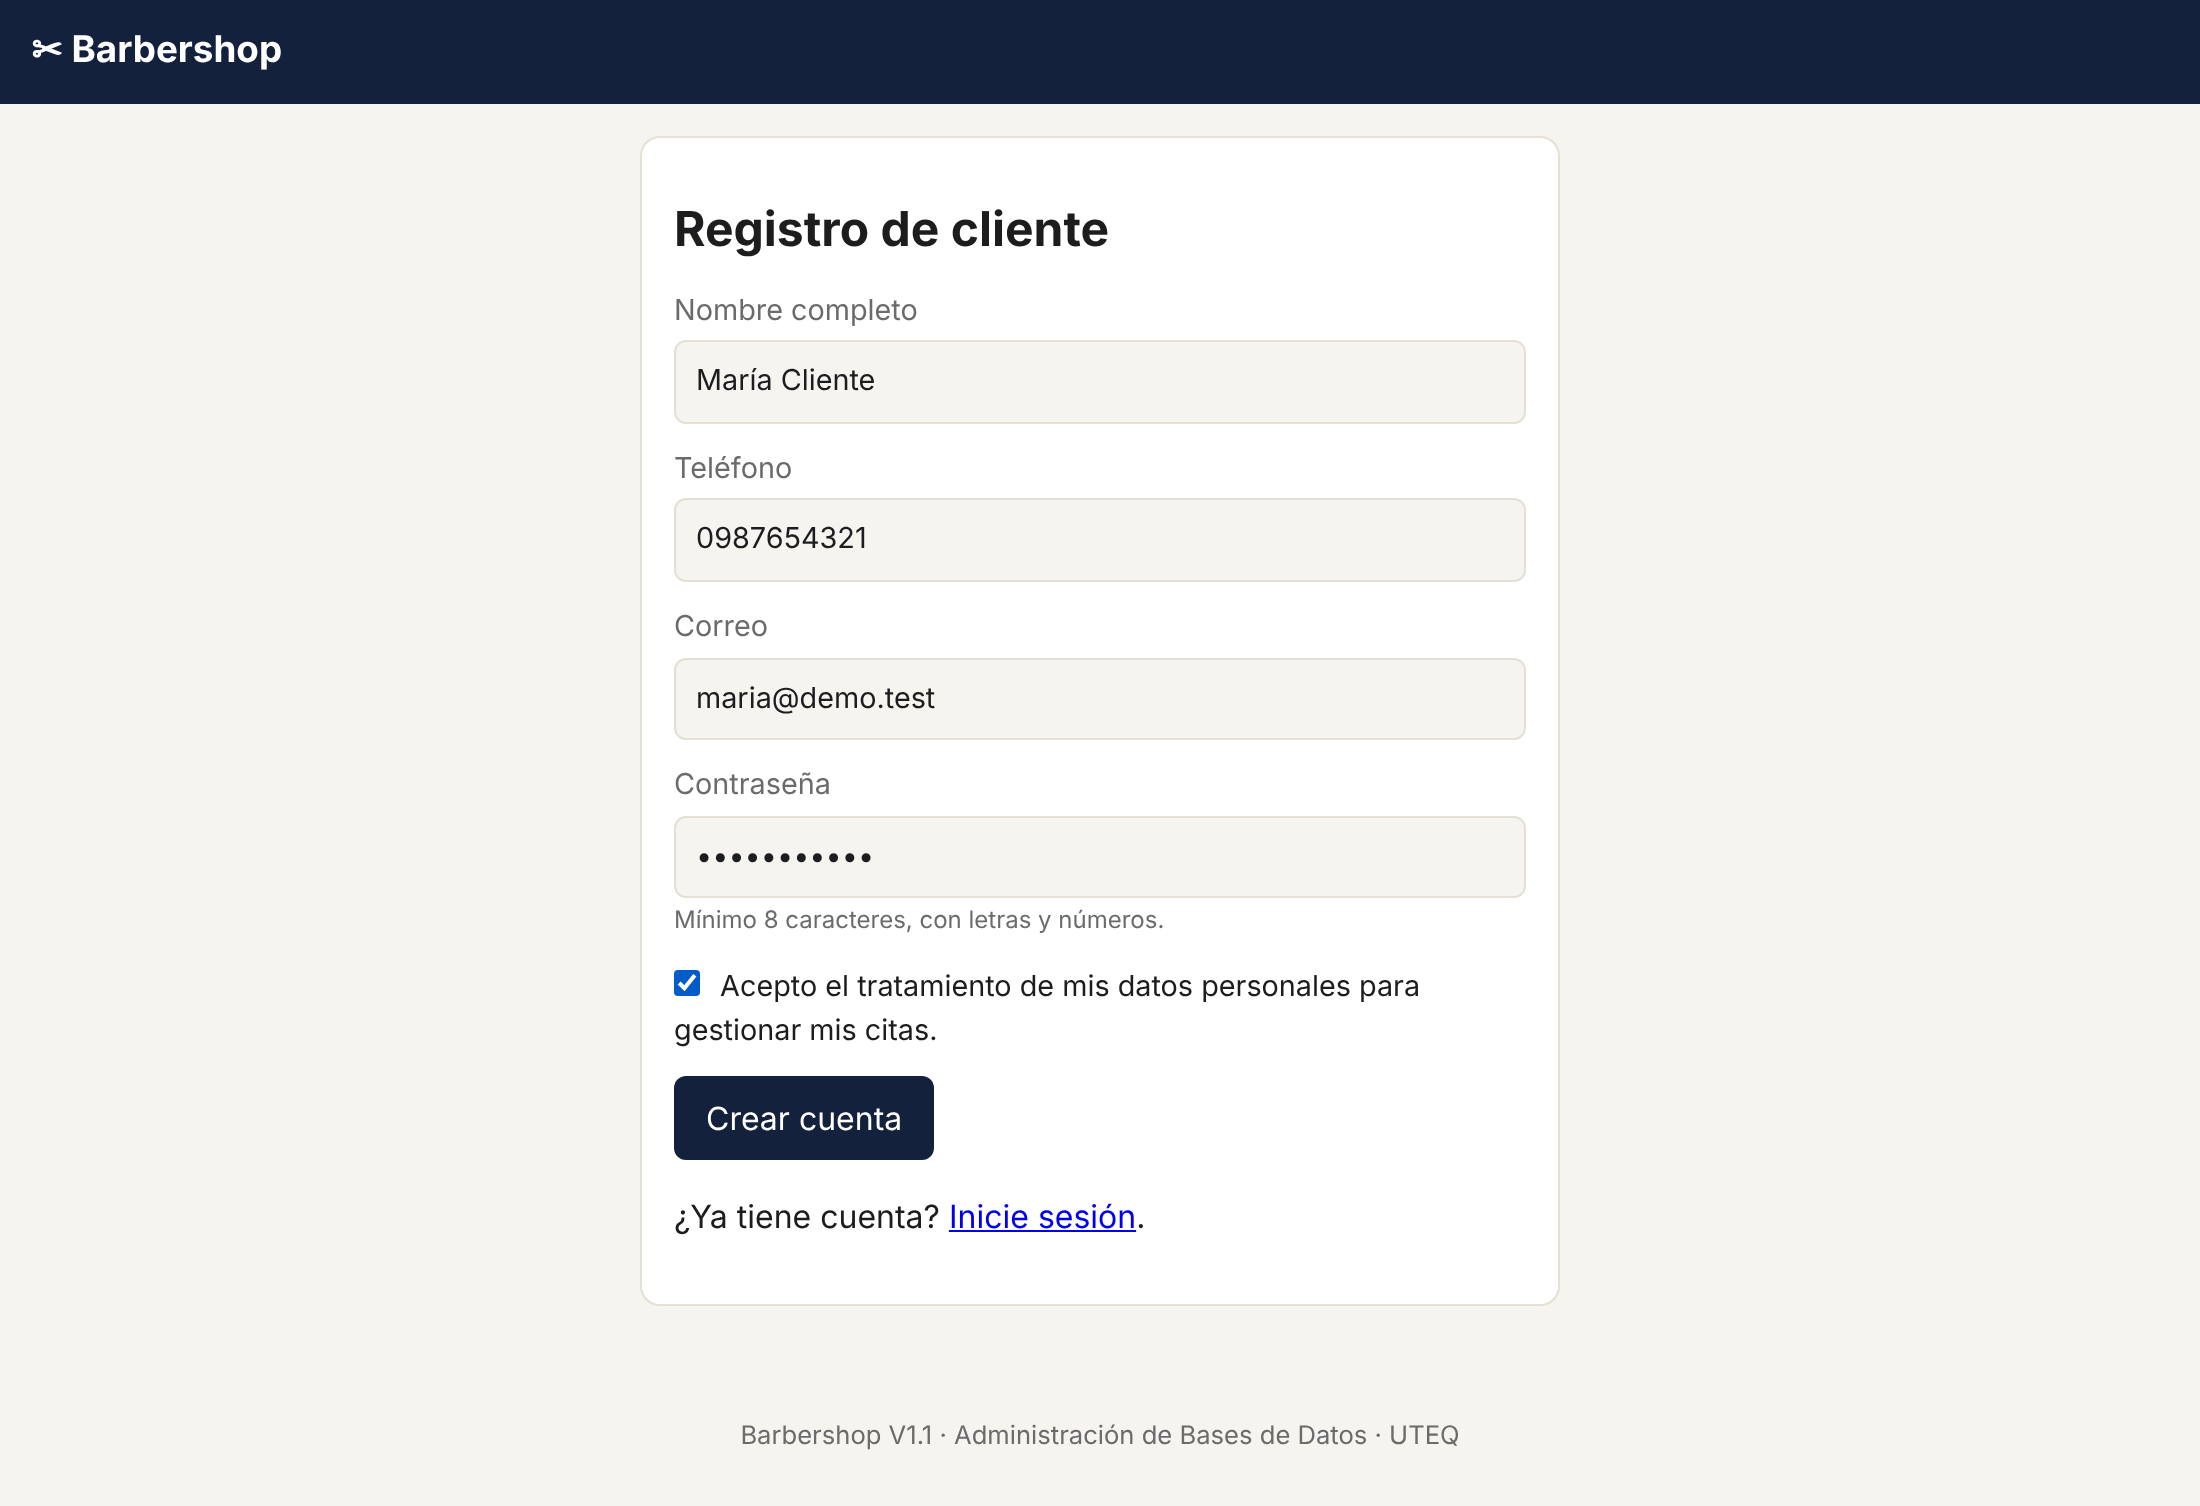
\includegraphics[width=.88\linewidth]{evidencias/fig1_registro.png}\caption{Registro de cliente (RF-01)}\end{figure}
\begin{figure}[H]\centering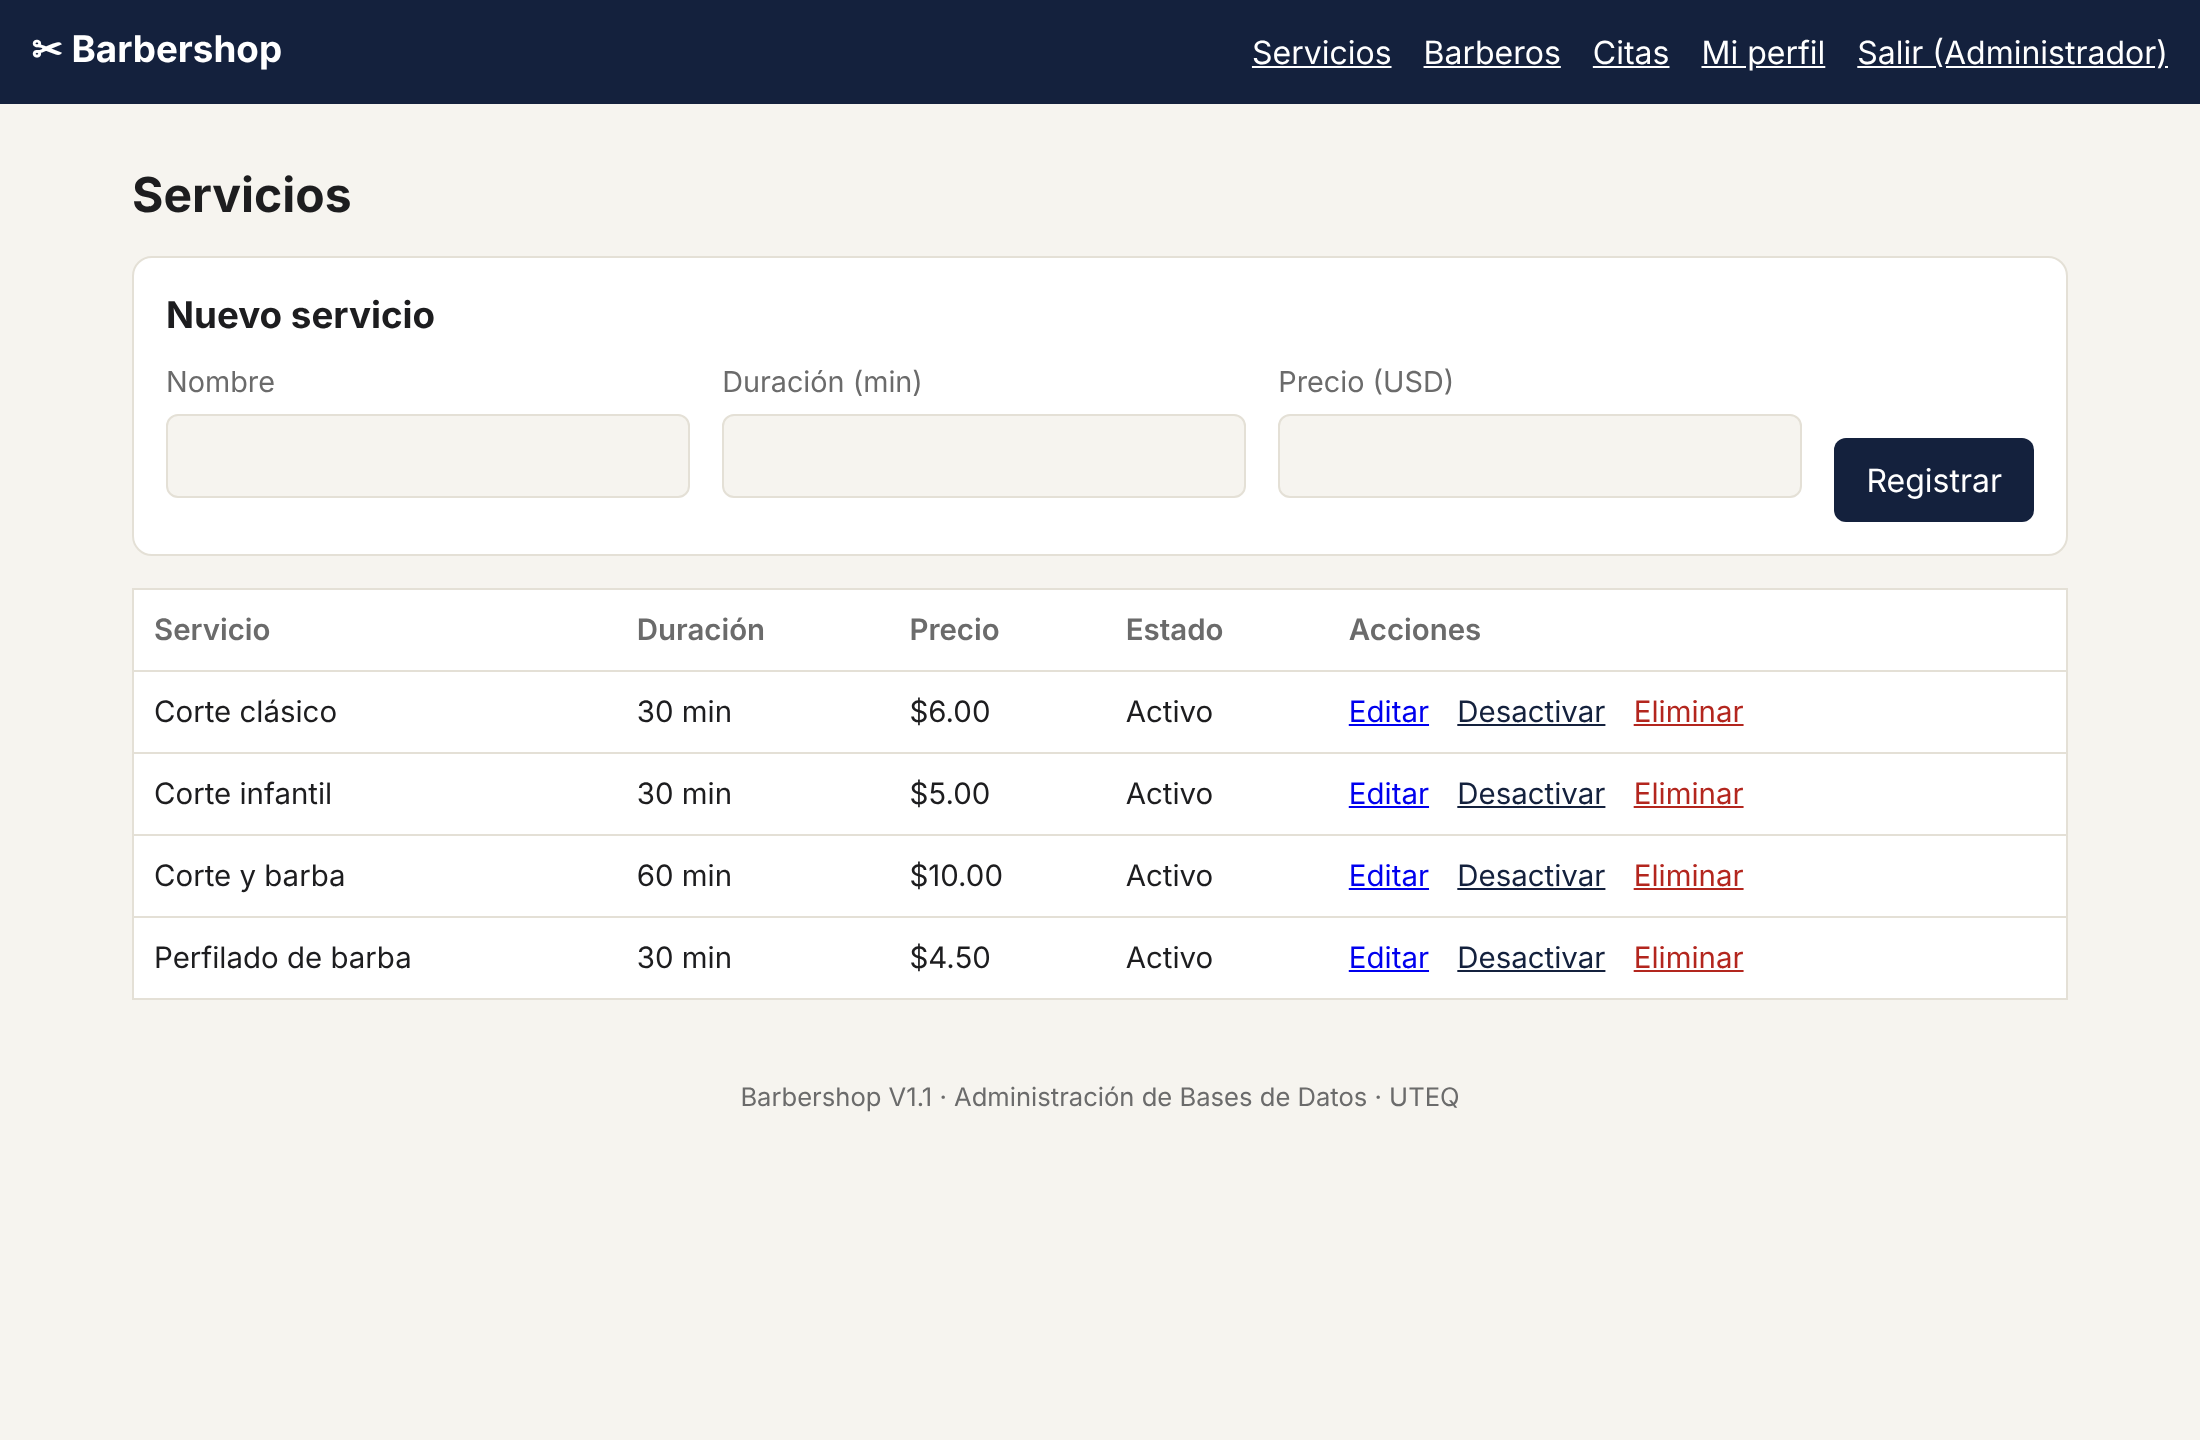
\includegraphics[width=.88\linewidth]{evidencias/fig2_servicios.png}\caption{CRUD de servicios para el administrador (RF-03)}\end{figure}
\begin{figure}[H]\centering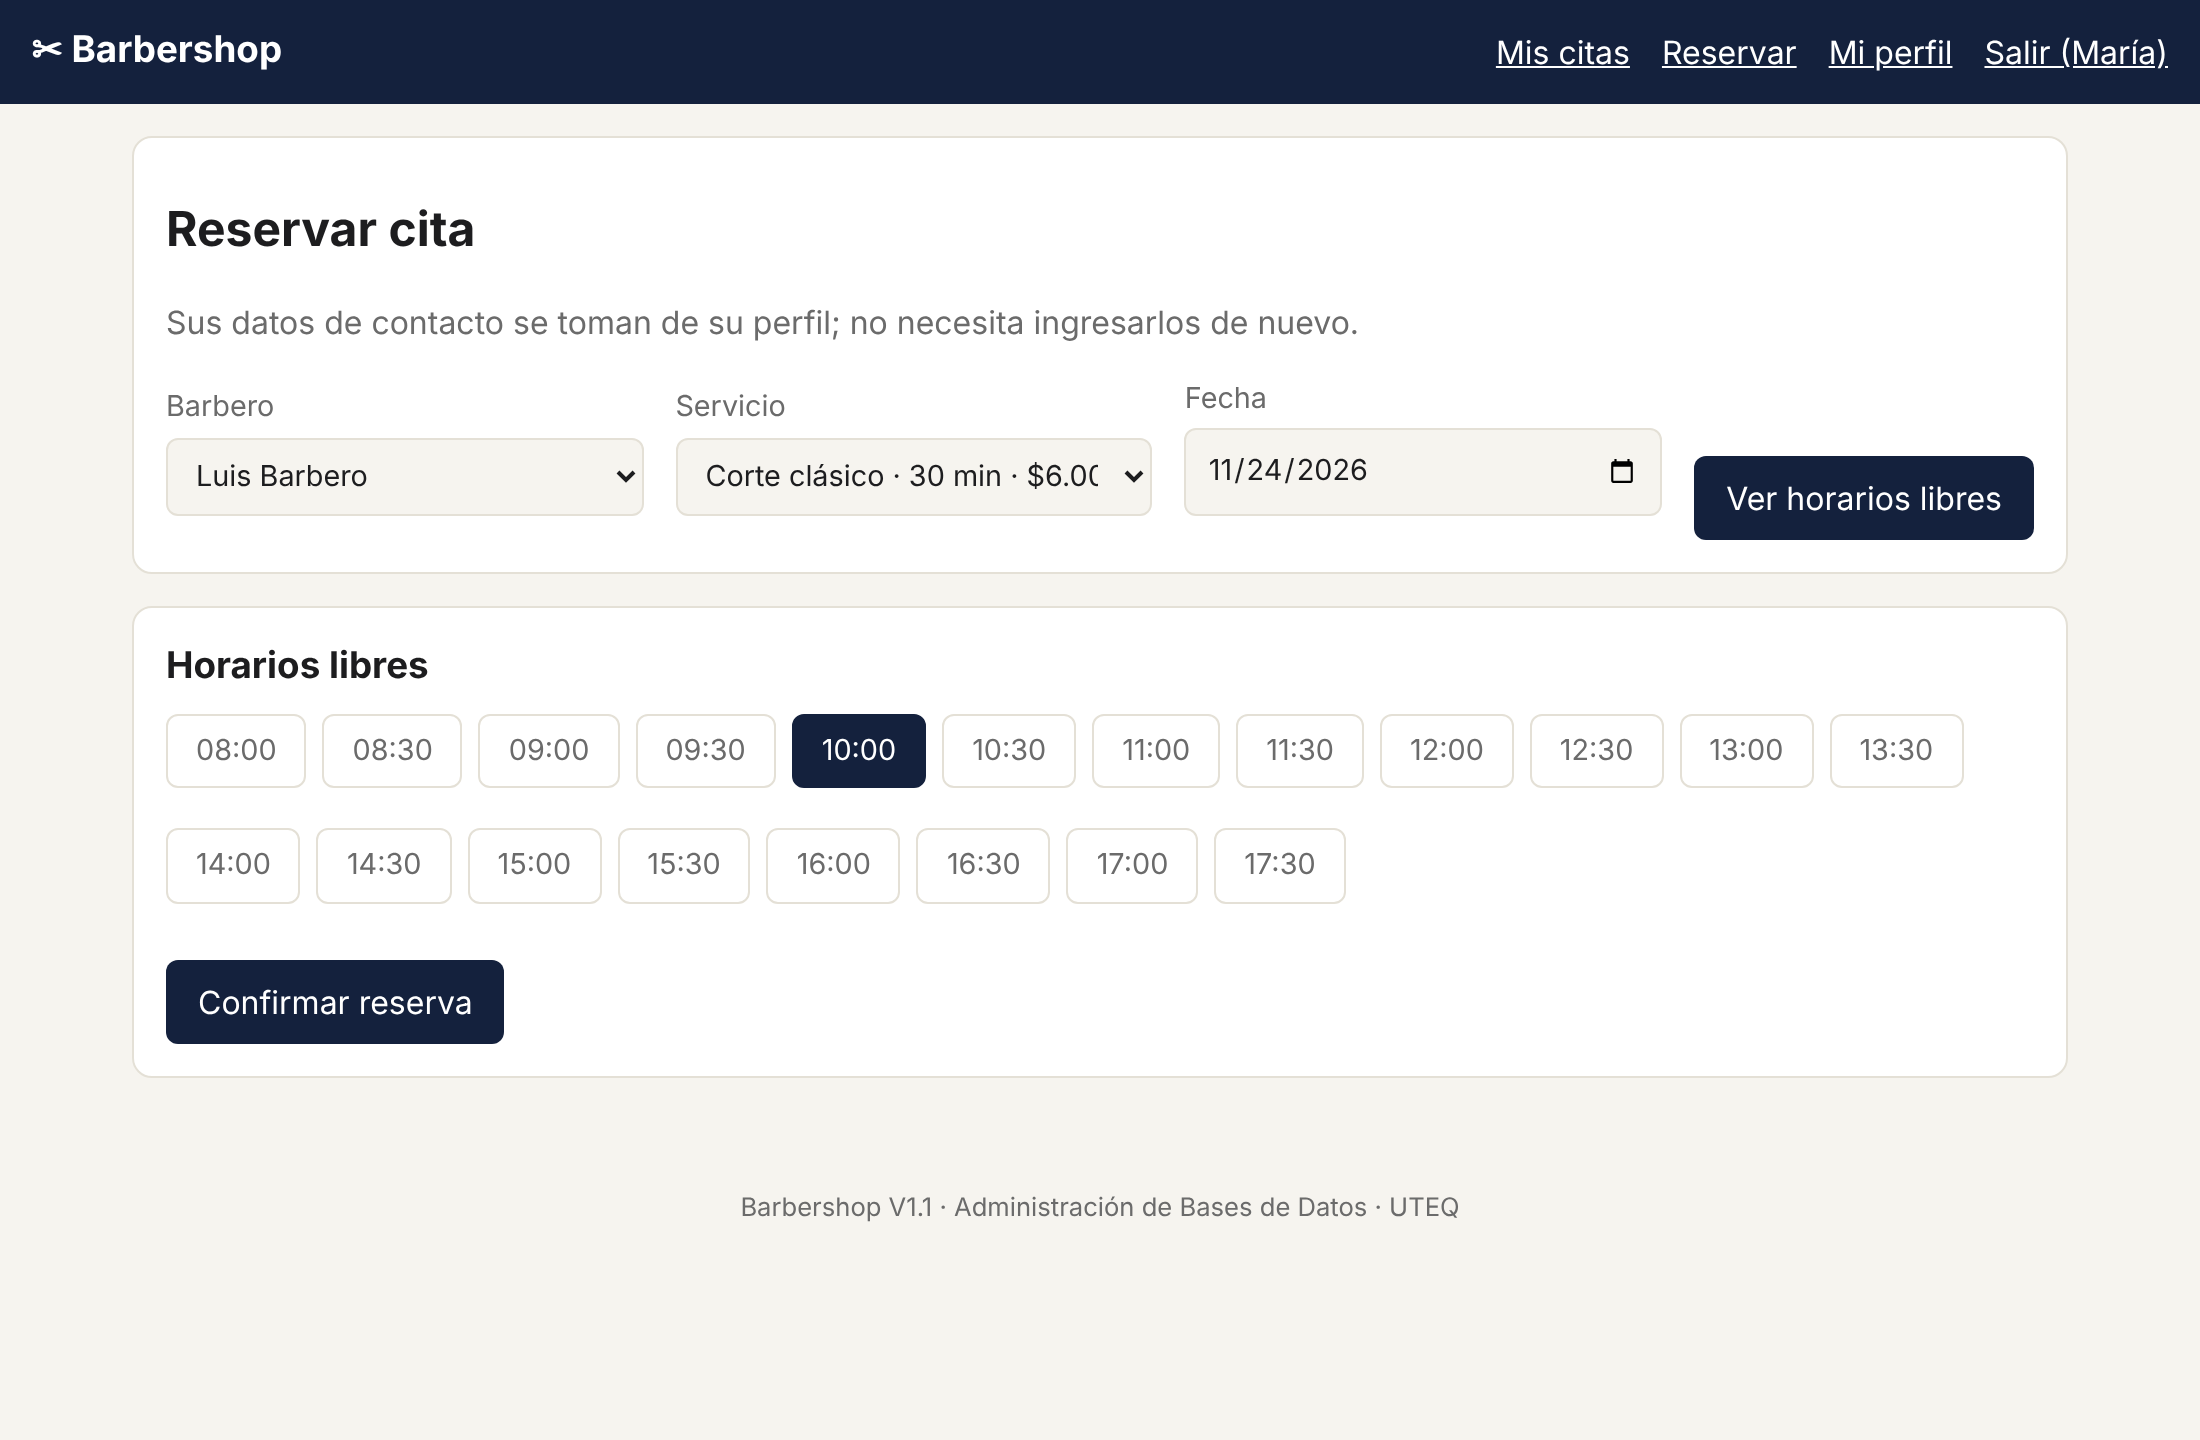
\includegraphics[width=.88\linewidth]{evidencias/fig3_reserva.png}\caption{Reserva con horarios libres (RF-04, RF-05)}\end{figure}
\begin{figure}[H]\centering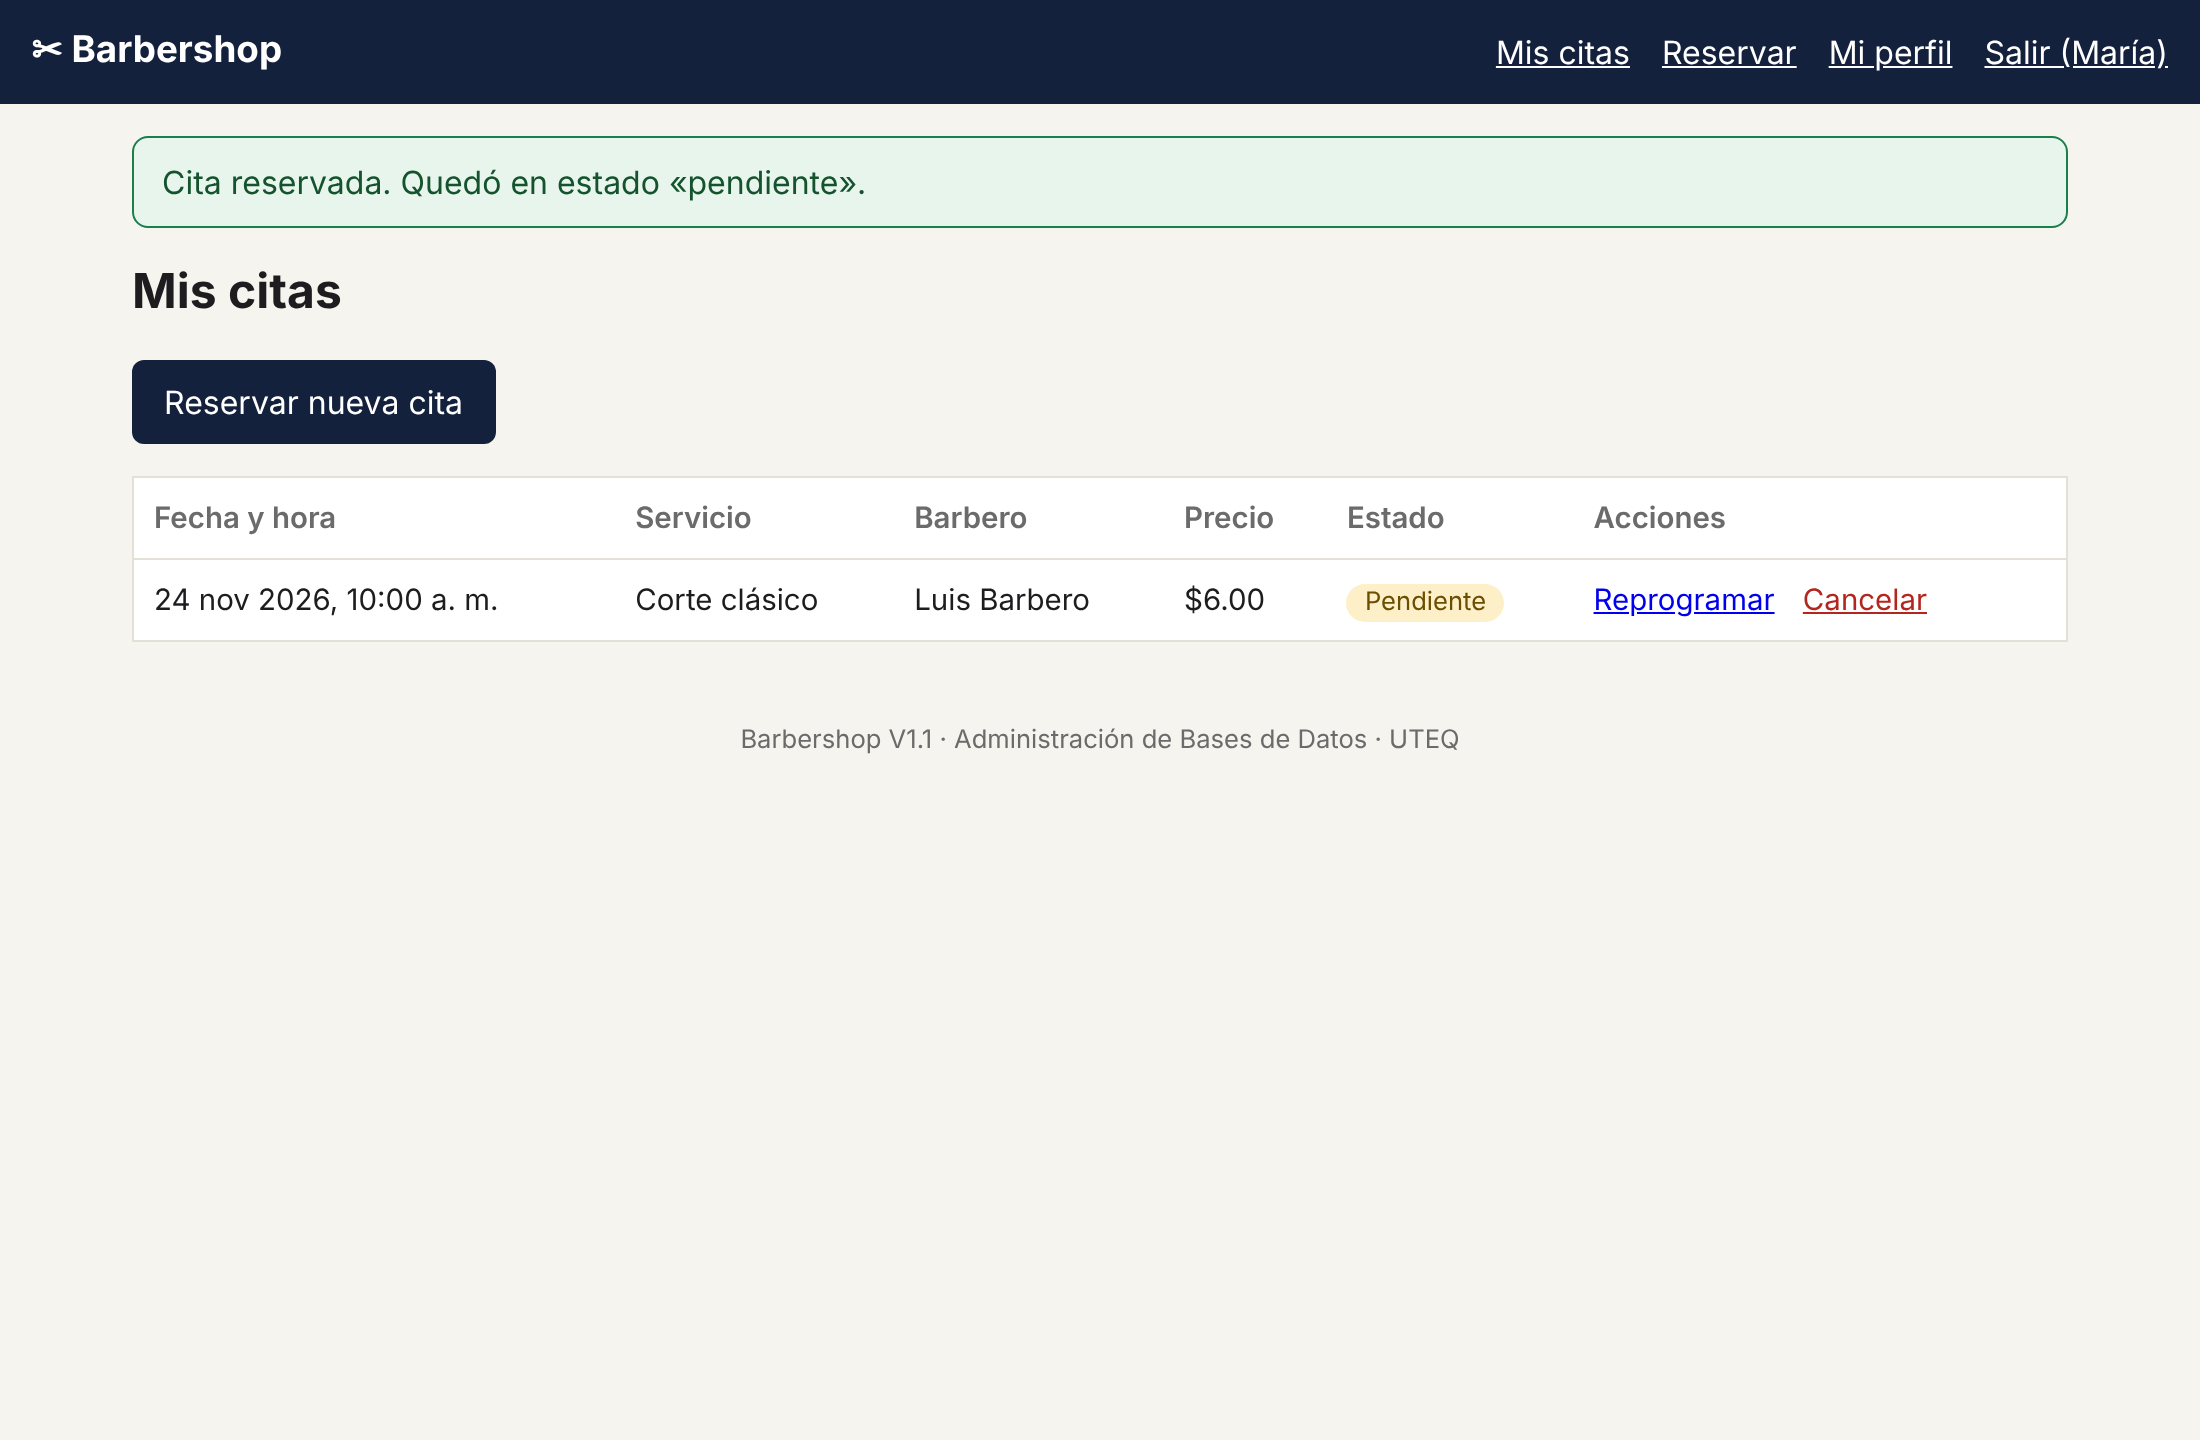
\includegraphics[width=.88\linewidth]{evidencias/fig4_mis_citas.png}\caption{Cita registrada en estado pendiente, con acciones de reprogramar y cancelar (RF-04, RF-06)}\end{figure}
\begin{figure}[H]\centering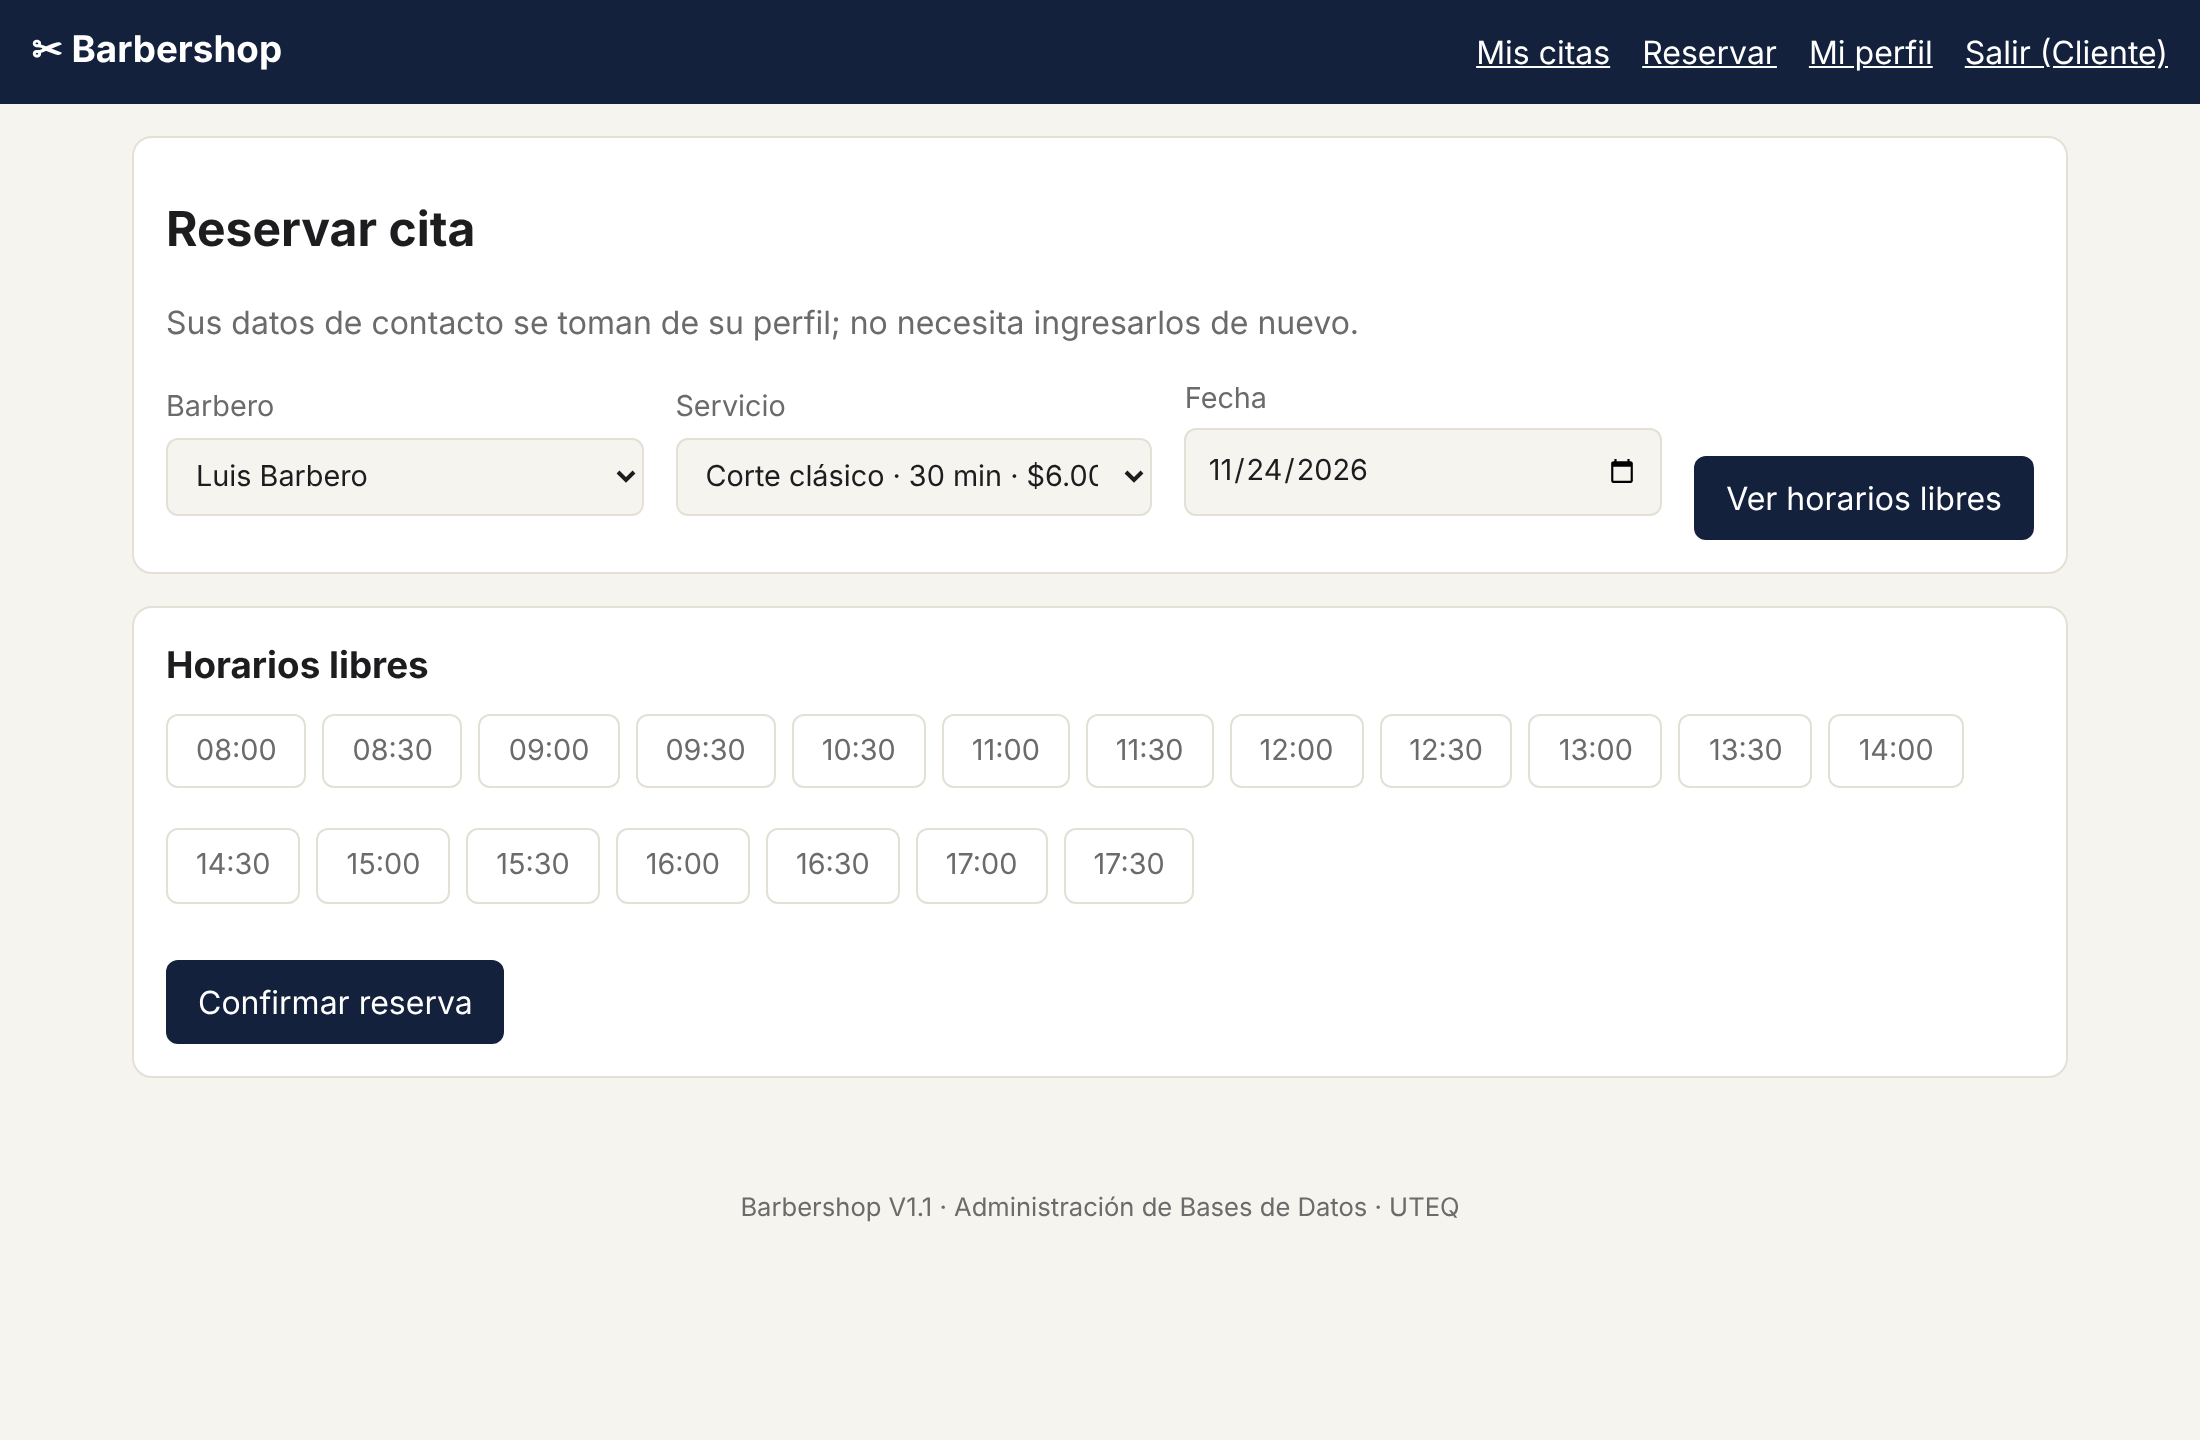
\includegraphics[width=.88\linewidth]{evidencias/fig5_horario_ocupado.png}\caption{Otro cliente: el horario de las 10:00 ya no se ofrece (RF-05)}\end{figure}
\begin{figure}[H]\centering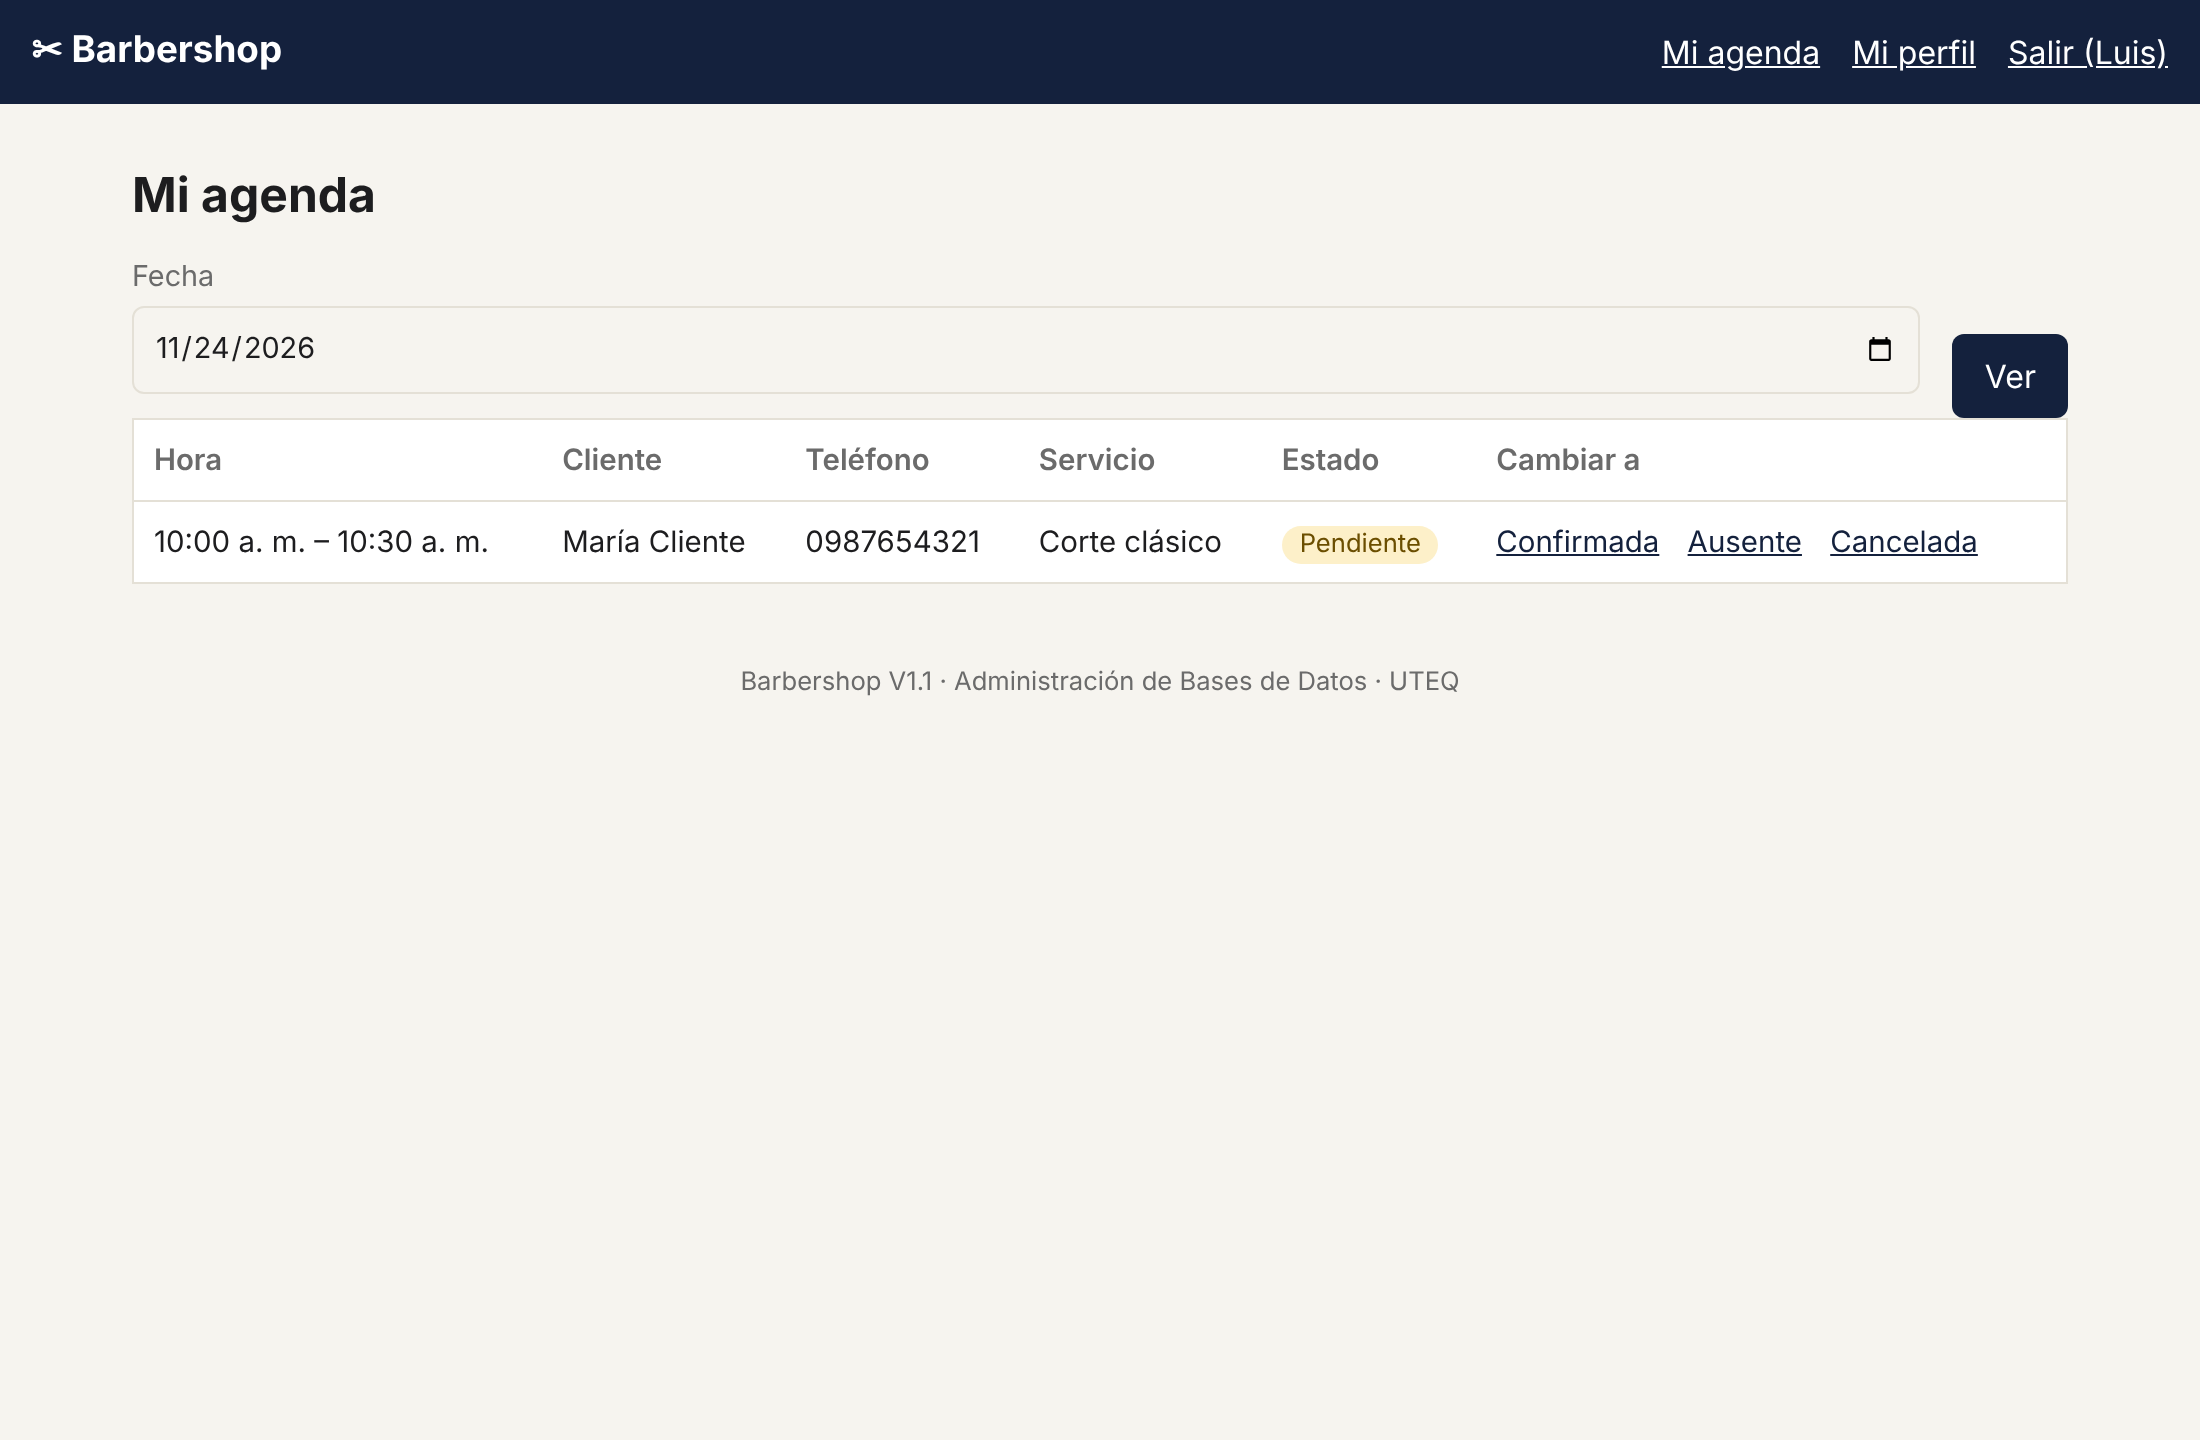
\includegraphics[width=.88\linewidth]{evidencias/fig6_agenda.png}\caption{Agenda del barbero con la cita y los cambios de estado permitidos (RF-07)}\end{figure}

\section{Pruebas funcionales}
Las pruebas se ejecutan con \texttt{npm test} (archivo \texttt{tests/run\_tests.js}). Cada caso realiza solicitudes HTTP a la aplicaci\'on y luego consulta PostgreSQL para comprobar que el cambio se refleje en la base. \textbf{Resultado de la \'ultima ejecuci\'on: 22 de 22 pruebas aprobadas} (PostgreSQL 16.15, Node.js 22).

{\footnotesize\setlength{\tabcolsep}{3pt}
\begin{longtable}{|>{\raggedright\arraybackslash}p{1.1cm}|>{\raggedright\arraybackslash}p{1.7cm}|>{\raggedright\arraybackslash}p{3.3cm}|>{\raggedright\arraybackslash}p{3.4cm}|>{\raggedright\arraybackslash}p{3.8cm}|>{\raggedright\arraybackslash}p{1.5cm}|}
\hline \textbf{ID} & \textbf{Req.} & \textbf{Datos} & \textbf{Esperado} & \textbf{Obtenido} & \textbf{Estado}\\\hline\endhead
PF-01 & RF-01 & nombre «Ana Pruebas», tel 0987654321, correo anamwqx0ax3@\allowbreak pruebas.test, clave válida, consentimiento & Cliente registrado (redirige a /login); en BD existe con rol cliente y contraseña con hash bcrypt & HTTP 302 $\rightarrow$ /login; BD: rol=cliente, hash=\$2b\$... & Aprobada \\ \hline
PF-02 & RF-01 & mismo correo anamwqx0ax3@\allowbreak pruebas.test en mayúsculas & Rechazado (HTTP 409) y sigue habiendo un solo registro & HTTP 409; registros con ese correo en BD: 1 & Aprobada \\ \hline
PF-03 & RF-01 & teléfono «abc», contraseña «123», sin consentimiento & Rechazado (HTTP 400) con mensajes de validación; no se inserta & HTTP 400; filas insertadas: 0 & Aprobada \\ \hline
PF-04 & RF-02 & credenciales válidas de cliente; luego clave errónea & Válidas: redirige a /citas. Erróneas: HTTP 401 & válidas: HTTP 302 $\rightarrow$ /citas; erróneas: HTTP 401 & Aprobada \\ \hline
PF-05 & RF-02 / RNF-03 & cliente$\rightarrow$\allowbreak/admin/\allowbreak servicios; barbero$\rightarrow$\allowbreak/admin/\allowbreak barberos; anónimo$\rightarrow$/citas & Cliente y barbero: HTTP 403; anónimo: redirige a /login & cliente: 403; barbero: 403; anónimo: 302 $\rightarrow$ /login & Aprobada \\ \hline
PF-06 & RNF-20 & 5 intentos fallidos y luego clave correcta & Cuenta bloqueada: HTTP 423 aun con la clave correcta; bloqueado\_hasta definido en BD & HTTP 423; bloqueado\_hasta=2026-11-21T21:38:28.215Z & Aprobada \\ \hline
PF-07 & Seguridad & correo «' OR '1'='1» en login; POST sin token CSRF & Inyección SQL sin efecto (HTTP 401); POST sin token rechazado (HTTP 403) & login inyectado: HTTP 401; POST sin CSRF: HTTP 403 & Aprobada \\ \hline
PF-08 & RF-03 & servicio «PRUEBA Barba», 20 min, \$4.50 & Creado; en BD con los valores indicados. Duración 0 y nombre repetido rechazados (400/409) & alta HTTP 302; BD: 20 min, \$4.50; duración 0: 400; duplicado: 409 & Aprobada \\ \hline
PF-09 & RF-03 / RNF-08 & cambiar precio de \$4.50 a \$5.25 & Precio actualizado y auditoría con usuario y valor anterior & precio BD \$5.25; auditoría: usuario=115, anterior=\{\textquotedbl{}precio\textquotedbl{}:4.5,\textquotedbl{}precio\_nuevo\textquotedbl{}:5.25\} & Aprobada \\ \hline
PF-10 & RF-03 & desactivar servicio y consultar formulario de reserva & Servicio inactivo en BD y ya no aparece en el formulario de reserva & activo=false; aparece en reserva: false & Aprobada \\ \hline
PF-11 & RF-03 & registrar barbero «Barbero Nuevo» con correo y clave inicial & Se crean usuario (rol barbero) y perfil de barbero; el barbero puede iniciar sesión & alta HTTP 302; BD rol=barbero, barbero\_id=15; login $\rightarrow$ /agenda & Aprobada \\ \hline
PF-12 & RF-04 & cliente B reserva barbero A, servicio 30 min, 2026-11-28 09:00 & Cita en estado «pendiente» asociada al cliente; el formulario no pide nombre, teléfono ni correo & HTTP 302; BD: estado=pendiente, 09:00--09:30; formulario pide datos personales: false & Aprobada \\ \hline
PF-13 & RF-05 / RN-01 & cliente C intenta barbero A, 2026-11-28 09:00 (ocupado) & Rechazado; sigue 1 sola cita activa en ese horario; el horario no figura entre los libres & HTTP 302; citas activas en ese horario: 1; 09:00 ofrecido: false; 09:30 ofrecido: true & Aprobada \\ \hline
PF-14 & RF-05 & cita de 30 min a las 09:15 (solapa con 09:00--09:30) & Rechazada por solape parcial; 1 sola cita activa en la franja & INSERT directo en SQL: rechazado por restricción EXCLUDE (23P01) & Aprobada \\ \hline
PF-15 & RF-06 & cliente B reprograma su cita a 2026-11-29 10:00; luego C reserva el horario anterior & Cita cambia de horario en BD y el horario anterior queda libre (C puede reservarlo) & reprogramación HTTP 302; BD: 2026-11-29 10:00; C reservó el horario liberado: true & Aprobada \\ \hline
PF-16 & RF-06 / RNF-08 & cliente B cancela su cita pendiente & Estado «cancelada»; horario libre; auditoría con usuario, fecha y valor anterior & HTTP 302; BD estado=cancelada; auditoría usuario=122, anterior=pendiente; 10:00 libre de nuevo: true & Aprobada \\ \hline
PF-17 & RF-06 & cita pendiente a 1 hora (plazo mínimo 2 h) y cancelación del cliente & Rechazada por plazo; la cita sigue «pendiente» en BD & HTTP 302; estado en BD: pendiente; mensaje de plazo mostrado: true & Aprobada \\ \hline
PF-18 & RF-06 & cliente C intenta cancelar la cita de otro cliente & No se modifica la cita ajena & estado de la cita ajena en BD: pendiente & Aprobada \\ \hline
PF-19 & RF-07 & barbero A consulta su agenda de 2026-11-28; barbero B consulta la suya & A ve la cita del cliente C; B no la ve & A ve la cita: true; B ve la cita: false & Aprobada \\ \hline
PF-20 & RF-07 & barbero A: pendiente$\rightarrow$confirmada; pendiente$\rightarrow$atendida; barbero B intenta cambiar cita de A & Primer cambio guardado; el salto inválido y el cambio ajeno se rechazan & tras confirmar: confirmada; tras salto inválido: confirmada; barbero B: HTTP 403, estado confirmada & Aprobada \\ \hline
PF-21 & RF-03 / RN-12 & eliminar servicio con citas y eliminar servicio sin citas & Con citas: no se elimina (se sugiere desactivar). Sin citas: se elimina & con citas: HTTP 302, sigue en BD: true; sin citas: HTTP 302, eliminado: true & Aprobada \\ \hline
PF-22 & RNF-13 / RN-01 & 20 clientes reservan a la vez barbero B, 2026-11-30 11:00 & Exactamente 1 solicitud aceptada; 1 sola cita activa en BD & solicitudes aceptadas: 1 de 20; citas activas en BD: 1 & Aprobada \\ \hline
\end{longtable}}

\section{Estado actualizado de la matriz de requisitos funcionales}
\begin{table}[H]\centering\small
\begin{tabularx}{\textwidth}{>{\raggedright\arraybackslash}p{1.7cm}>{\raggedright\arraybackslash}p{2.6cm}>{\raggedright\arraybackslash}p{3.2cm}Y}\toprule
\textbf{Requisito} & \textbf{Estado} & \textbf{Funcionalidad} & \textbf{Evidencia}\\\midrule
RF-01 & Completado & \texttt{/registro}, \texttt{/perfil} & PF-01 a PF-03; Fig. 1\\
RF-02 & Completado (parcial en RNF-20) & \texttt{/login} & PF-04 a PF-07\\
RF-03 & Completado & \texttt{/admin/servicios}, \texttt{/admin/barberos} & PF-08 a PF-11, PF-21; Fig. 2\\
RF-04 & Completado & \texttt{/citas/nueva} & PF-12; Fig. 3 y 4\\
RF-05 & Completado & Restricci\'on \texttt{ex\_citas\_sin\_cruce} & PF-13, PF-14, PF-22; Fig. 5\\
RF-06 & Completado, salvo citas pagadas (RF-68) & \texttt{/citas} & PF-15 a PF-18\\
RF-07 & Completado & \texttt{/agenda} & PF-19, PF-20; Fig. 6\\
RF-19 & En desarrollo (horario global por configuraci\'on) & \texttt{HORA\_APERTURA}, \texttt{HORA\_CIERRE} & ---\\
RF-08, RF-09, RF-10, RF-11, RF-14, RF-15, RF-16, RF-17, RF-41, RF-68 & Pendiente (V1.1) & --- & ---\\
RF-21, RF-25, RF-26, RF-28, RF-29, RF-44 & Pendiente (V1.2) & --- & ---\\\bottomrule
\end{tabularx}
\caption{Estado de los 24 requisitos funcionales de la V1: 7 completados, 1 en desarrollo, 16 pendientes}\end{table}

\section{Distribuci\'on del trabajo del equipo}
El trabajo se dividi\'o por m\'odulos y carpetas del repositorio, de modo que cada integrante es responsable de una parte del c\'odigo y de sus propios commits en GitHub (\href{https://github.com/ramaguas-ship-it/Barbershop}{\textcolor{azul}{github.com/ramaguas-ship-it/Barbershop}}). La Tabla~\ref{tab:reparto} resume la labor de cada uno.
\begin{table}[H]\centering\footnotesize
\begin{tabularx}{\textwidth}{>{\raggedright\arraybackslash}p{2.7cm}>{\raggedright\arraybackslash}p{4.6cm}>{\raggedright\arraybackslash}p{2.3cm}Y}\toprule
\textbf{Integrante} & \textbf{Labor realizada} & \textbf{Requisitos} & \textbf{Carpetas y archivos} \\ \midrule
Amagua Sac\'on Robyn Willian & Dise\~no del esquema PostgreSQL (tablas, claves for\'aneas, restricci\'on contra cruces de horario, auditor\'ia), datos de demostraci\'on y entorno con Docker. & RF-05, RNF-08 & \texttt{db/}, \texttt{scripts/}, \texttt{docker-compose.yml}, \texttt{.env.example}, \texttt{.gitignore} \\
Barrionuevo Fuentes Carlos Daniel & Servidor Express, conexi\'on parametrizada a PostgreSQL, sesiones, token CSRF, control de acceso por rol, registro, perfil e inicio de sesi\'on. & RF-01, RF-02, RNF-20 & \texttt{src/app.js}, \texttt{config.js}, \texttt{db.js}, \texttt{middleware/}, \texttt{routes/auth.js}, \texttt{views/auth/}, \texttt{views/partials/}, \texttt{package.json} \\
Marcillo Ponce Alberto Jeanpool & Administraci\'on de servicios y barberos (crear, consultar, actualizar y eliminar), validaciones y auditor\'ia de cambios de precio. & RF-03 & \texttt{src/routes/admin.js}, \texttt{src/views/admin/} \\
Mes\'ias Quijije Jhon Alexander & Reserva, reprogramaci\'on y cancelaci\'on de citas, c\'alculo de horarios libres y agenda del barbero con cambio de estado; estilos de la interfaz. & RF-04, RF-05, RF-06, RF-07 & \texttt{src/services.js}, \texttt{routes/citas.js}, \texttt{routes/agenda.js}, \texttt{views/citas/}, \texttt{public/estilos.css} \\
Vera G\'omez Anthony Alfredo & 22 pruebas funcionales con verificaci\'on en PostgreSQL, informe t\'ecnico en LaTeX, matriz de requisitos, evidencias y README. & PF-01 a PF-22 & \texttt{tests/}, \texttt{informe/}, \texttt{README.md} \\ \bottomrule
\end{tabularx}
\caption{Reparto de labores por integrante}\label{tab:reparto}\end{table}
Cada carpeta del repositorio tiene un solo responsable, lo que evita conflictos al combinar los cambios y permite ver en GitHub la contribuci\'on individual (Insights $\rightarrow$ Contributors).

\section{Dificultades t\'ecnicas y decisiones adoptadas}
\begin{table}[H]\centering\small
\begin{tabularx}{\textwidth}{>{\raggedright\arraybackslash}p{4.2cm}YY}\toprule
\textbf{Dificultad} & \textbf{Causa} & \textbf{Decisi\'on o soluci\'on}\\\midrule
El script de datos de demostraci\'on fall\'o con \emph{value too long for type character varying(10)} & La columna \texttt{rol} ten\'ia 10 caracteres y \emph{administrador} tiene 13 & Se ampli\'o a \texttt{VARCHAR(15)} y se recre\'o la base; la prueba con datos semilla detect\'o el error antes de la entrega\\
Evitar cruces con solicitudes simult\'aneas & Validar solo en la aplicaci\'on deja una ventana entre consultar y guardar & La garant\'ia se traslad\'o a PostgreSQL con \texttt{EXCLUDE} y \texttt{btree\_gist}; la aplicaci\'on solo captura el error \texttt{23P01} y avisa al usuario\\
Las p\'aginas de error no cargaban (\emph{user is not defined}) & El middleware CSRF respond\'ia antes de definir las variables de las vistas & Se reorden\'o el middleware y se hizo robusto el encabezado\\
Horarios y zona horaria & Los horarios se comparan en la hora local, pero se guardan en UTC & Columnas \texttt{timestamptz} y conversi\'on expl\'icita a \texttt{America/Guayaquil} en las consultas\\
Eliminar registros con historial (RN-12) & Las claves for\'aneas impiden borrar servicios o barberos con citas & Se mantuvo \texttt{ON DELETE RESTRICT}; la interfaz informa y sugiere desactivar\\
Versi\'on de PostgreSQL de las pruebas & Las pruebas se ejecutaron en un entorno con PostgreSQL 16, no con la imagen 18 del contenedor del equipo & El SQL usado es est\'andar y compatible con 18, pero el equipo debe repetir \texttt{npm test} sobre su contenedor y anexar esa evidencia\\\bottomrule
\end{tabularx}
\caption{Dificultades y decisiones}\end{table}
Ninguna de estas decisiones modifica los objetivos, el alcance ni los requisitos de la especificaci\'on de la semana 2.

\section{Conclusiones}
La primera versi\'on permite registrar, consultar, actualizar y eliminar servicios, barberos y citas desde una interfaz web conectada a PostgreSQL, con validaciones y mensajes de resultado. La regla central del negocio, no reservar un horario ocupado, se aplica dentro de la base de datos y resiste solicitudes simult\'aneas. Quedan pendientes el pago en l\'inea, el cobro, la caja y el inventario, que dependen de esta base y son la siguiente prioridad.
\end{document}
